\documentclass{article}

\usepackage{polski}
\usepackage{amsmath}
\usepackage{graphicx}
\usepackage{float}
\usepackage{subfig}
\usepackage{multirow}

\title{Interpolacja funkcjami sklejanymi}
\author{\textbf{Łukasz Wala}\\
    \textit{AGH, Wydział Informatyki, Elektroniki i Telekomunikacji} \\
    \textit{Metody Obliczeniowe w Nauce i Technice 2021/2022}}
\date{Kraków, \today}

\begin{document}
\maketitle

\section{Opis problemu}
Główną ideą zadania jest zbadanie zachowania wielomianów interpolacyjnych
dla poniższej funkcji skonstruowanych za pomocą funkcji sklejanych drugiego oraz
trzeciego stopnia dla różnych warunków brzegowych.

Badana funkcja:
\[f(x)=x^2-m\cdot\cos\left(\frac{\pi x}{k}\right)\]
Gdzie $k=\frac{1}{2}$, $m=4$ oraz $x\in [-6,6]$.

\section{Opracowanie}
\subsection{Wielomiany interpolacyjne}
Do skonstruowanie wielomianów i narysowania wykresów zostanie użyty załączony program w języku Python.
Pierwszym krokiem będzie zbadanie zachowanie i różnic pomiędzy wielomianami sklejanymi drugiego oraz trzeciego 
stopnia. Różnice wynikające z zmiany warunków brzegowych zostaną zbadane w kolejnej sekcji. Tutaj zostaną użyte:
\begin{itemize}
    \item
    dla wielomianów 3 stopnia - przybliżanie trzecich pochodnych w pierwszym i ostatnim punkcie ilorazami różnicowymi,
    \item
    dla wielomianów 2 stopnia - przybliżanie pierwszych pochodnych w pierwszym punkcie ilorazem różnicowym.
\end{itemize}

Zakres liczb węzłów, dla których badane będą wielomiany wynosi 4-50. Wezły rozłożone są równomiernie, ponieważ, 
jako że stopnie wielomianów są niewielkie, nie występuje efekt Rungego.

\begin{figure}[H]
    \centering
    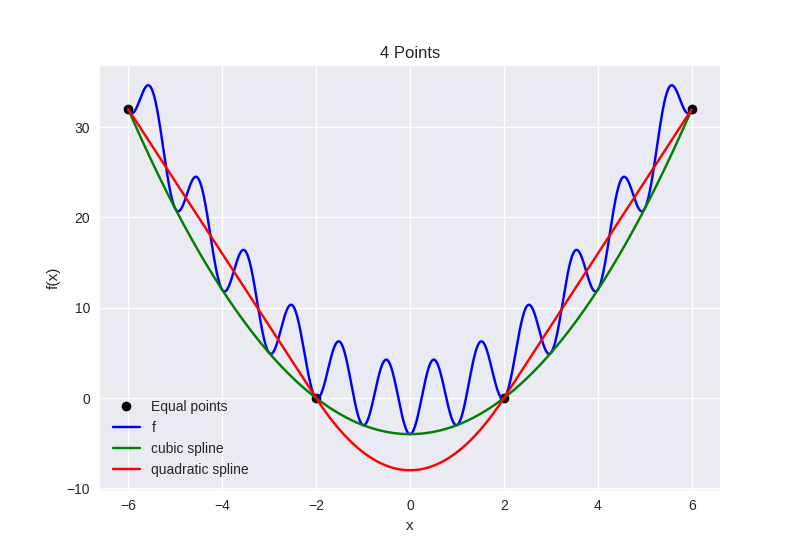
\includegraphics[width=\textwidth]{img/spline_4.png}
    \caption{Interpolacja splajnami dla 4 punktów}
\end{figure}

\begin{figure}[H]
    \centering
    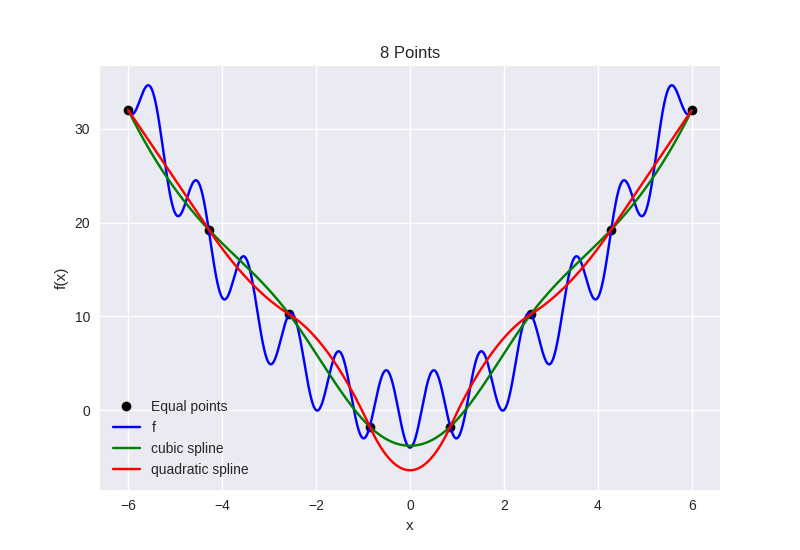
\includegraphics[width=\textwidth]{img/spline_8.png}
    \caption{Interpolacja splajnami dla 8 punktów}
\end{figure}

Dla 9 węzłów w przypadku wielomianów 2 stopnia pojawiają się oscylacje, może być to spowodowane
wachającymi się wartościami funkcji w węzłach. Warto również zauważyć, że oscylacja występuje po prawej stronie wykresu, 
ponieważ dla lewego krańca określony jest warunek brzegowy. W przypadku wielomianów 3 stopnia podobny problem nie występuje.

\begin{figure}[H]
    \centering
    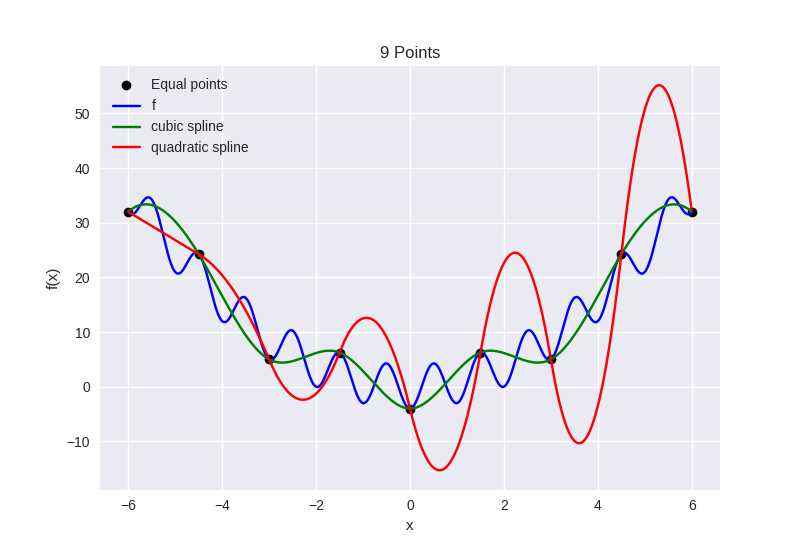
\includegraphics[width=0.8\textwidth]{img/spline_9.png}
    \caption{Interpolacja splajnami dla 9 punktów}
\end{figure}

\begin{figure}[H]
    \centering
    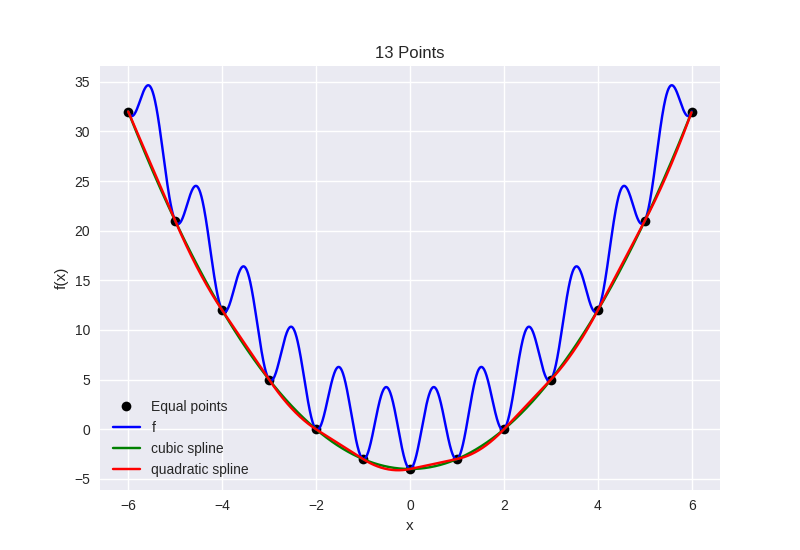
\includegraphics[width=0.8\textwidth]{img/spline_13.png}
    \caption{Interpolacja splajnami dla 13 punktów}
\end{figure}

Dla kolejnych liczb węzłów (większych niż 9) efekt oscylacji nie pojawia się, wielomiany zachowują się przewidywalnie.
Podobny problem pojawia się w okolicy liczby 22 węzłów. Tutaj, z racji dużej liczby węzłów, warunek brzegowy nie wpływa na obszar oscylacji.
Dla wielomianów 3 stopnia, podobnie jak w poprzednim przypadku, efekt nie występuje, poprawnie przybliżają badaną funkcję.

\begin{figure}[H]
    \centering
    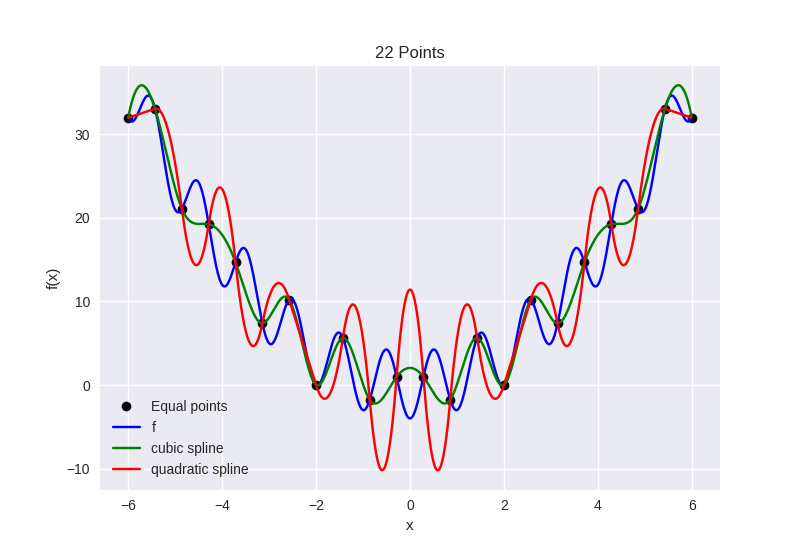
\includegraphics[width=0.8\textwidth]{img/spline_22.png}
    \caption{Interpolacja splajnami dla 22 punktów}
\end{figure}

\begin{figure}[H]
    \centering
    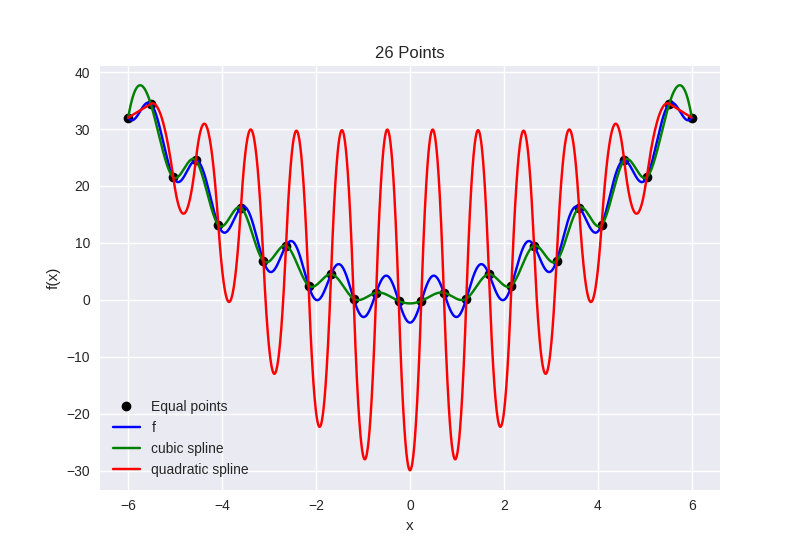
\includegraphics[width=0.8\textwidth]{img/spline_26.png}
    \caption{Interpolacja splajnami dla 26 punktów}
\end{figure}

Oscylacja nasila się od liczby 26 węzłów, następnie efekt maleje, a wielomniany 2 stopnia coraz lepije przybliżają badaną funkcję.

\begin{figure}[H]
    \centering
    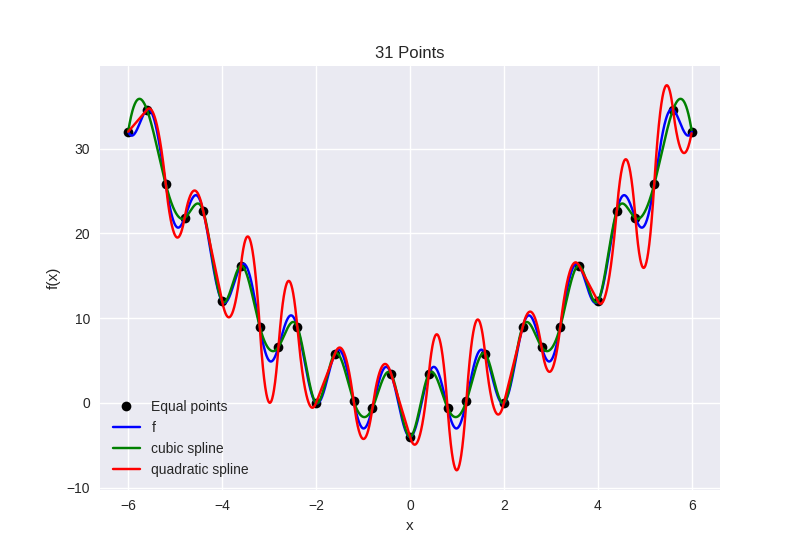
\includegraphics[width=\textwidth]{img/spline_31.png}
    \caption{Interpolacja splajnami dla 31 punktów}
\end{figure}

\begin{figure}[H]
    \centering
    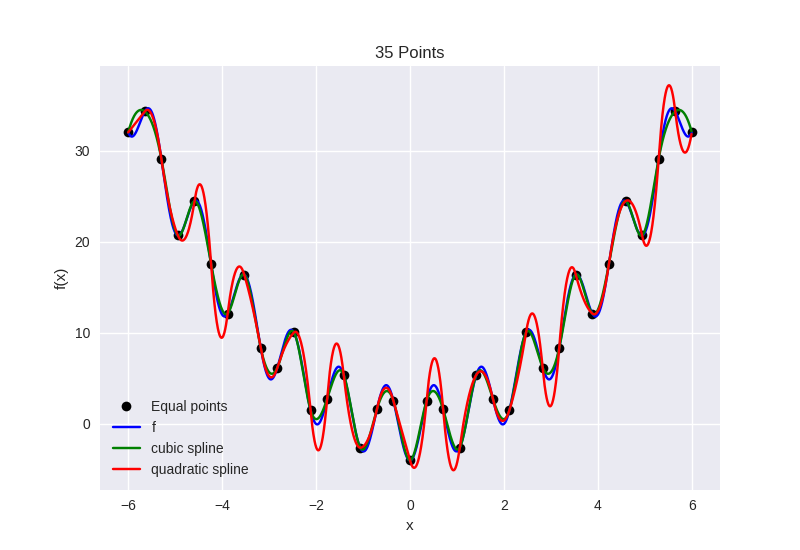
\includegraphics[width=\textwidth]{img/spline_35.png}
    \caption{Interpolacja splajnami dla 35 punktów}
\end{figure}

Na wykresie dla 35 punktów można zauważyć, że przybliżenie jest relatywnie dokładne dla wielomianów 3 stopnia oraz niewiele mniej dokładne
dla wielomianów 2 stopnia.

\begin{figure}[H]
    \centering
    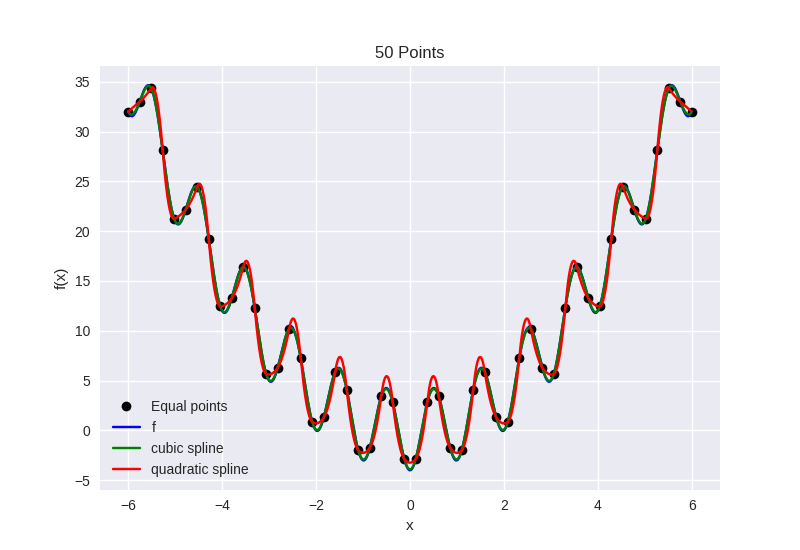
\includegraphics[width=\textwidth]{img/spline_50.png}
    \caption{Interpolacja splajnami dla 50 punktów}
\end{figure}

\subsection{Warunki brzegowe}
Zarówno dla wielomianów interpolowanych sklejanymi funkcjami trzeciego jak i drugiego stopnia zbadano dwa rodzaje warunków brzegowych:
\begin{itemize}
    \item
    dla wielomianów trzeciego stopnia:
    \begin{itemize}
        \item
        warunek 1 - przybliżanie trzecich pochodnych w pierwszym i ostatnim węźle ilorazami różnicowymi,
        \item
        warunek 2, free boundary - drugie pochodne w pierwszym i ostatnim węźle zastąpione zerami,
    \end{itemize}
    \item
    dla wielomianów drugiego stopnia:
    \begin{itemize}
        \item
        warunek 1 - przybliżanie pierwszej pochodnej w pierwszym węźle ilorazem różnicowymi,
        \item
        warunek 2 - zastąpienie pierwszej pochodnej w pierwszym węźle zerem,
    \end{itemize}
\end{itemize}

\subsection{Dokładność}
Pozostaje obliczenie dokładności oraz skonfrontowanie wyników z wnioskami uzyskanymi na podstawie analizy wykresów. Miarami dokładności będą:
\begin{itemize}
    \item
    Średnia kwadratów odległości wartości wielomianu oraz funkcji $f$ dla 1000 równo oddalonych punktów,
    \item
    Maksymalna odległość wartości wielomianu oraz funkcji $f$ dla 1000 równo oddalonych punktów.
\end{itemize}

\section{Wnioski}


\end{document}